\chapter{Installation instruction}
\label{appendix:B}
\section{Windows}
\begin{enumerate}
    \item Install Docker for Windows using instructions from: \newline
    \url{https://docs.docker.com/docker-for-windows/install/}
    \item Enable hyper-v using instructions from: \newline
    \url{https://docs.microsoft.com/en-us/virtualization/hyper-v-on-windows/quick-start/enable-hyper-v}
    \item Restart the computer
    \item Click Docker icon in tray and enable option "Switch to Linux Containers..." \newline
        \begin{minipage}{\linewidth}
            \centering
        	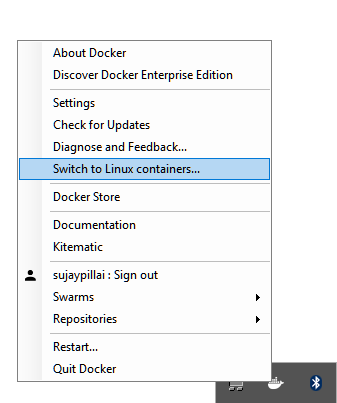
\includegraphics[width=0.4\linewidth]{instructions/systemtray.png}
        \end{minipage}
    \item Optional - open docker settings by clicking settings option and  in advanced settings adjust how much resources can docker containers use
    \newline
        \begin{minipage}{\linewidth}
            \centering
        	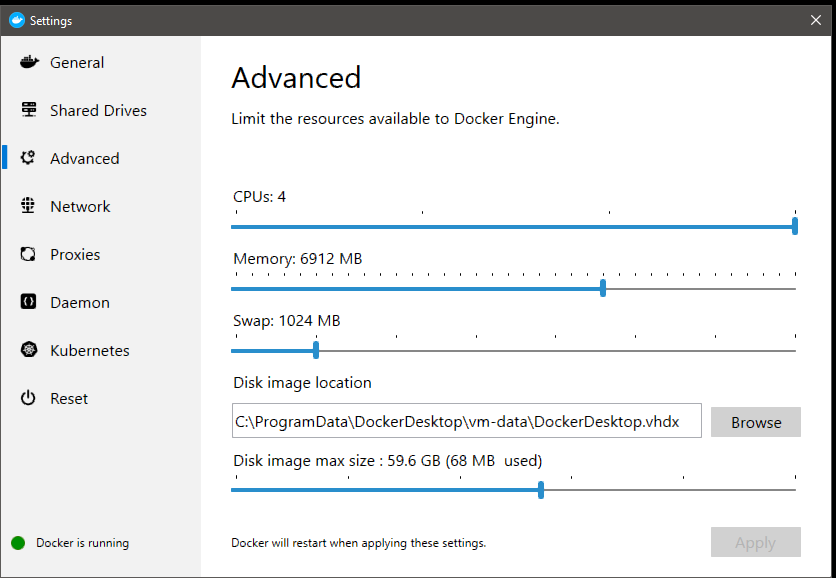
\includegraphics[width=0.4\linewidth]{instructions/res.PNG}
        \end{minipage}
    \item Clone or download repository from: \newline
     \url{https://github.com/JakubSokolowski/simbad-monorepo}
    \item Open \textit{PowerShell} by pressing windows+R, typing "powershell" and pressing enter.
    \item From inside of  \textit{PowerShell} change directory to directory when the cloned repository is. The easiest way to do that is to find folder containing repository in Windows Explorer, type "cd " in  \textit{PowerShell} and drag and drop this folder onto  \textit{PowerShell} window. The command in  \textit{PowerShell} should now look like "cd C:\textbackslash Users\textbackslash Alice\textbackslash simbad\-monorepo". Press enter to execute it.
    \item While in cloned folder, enter command docker-compose -f docker/prod-docker-compose.yml up. This will start the download process - this operation may take around 15 mins depending on the internet connection and will download around 4GB of data. \newline
        \begin{minipage}{\linewidth}
            \centering
        	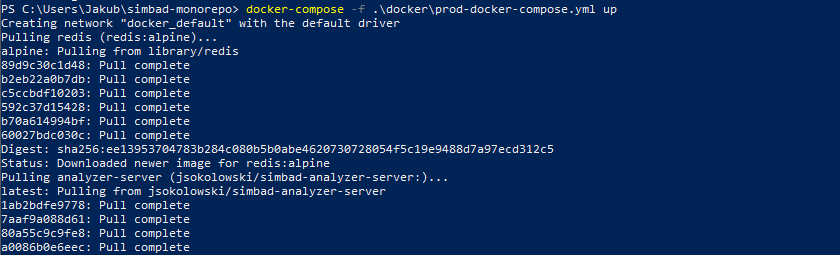
\includegraphics[width=0.9\linewidth]{instructions/docker2.PNG}
        \end{minipage}
    \item Docker will prompt you to enter password for, to grant access to host filesystem. Enter user password for each such prompt. \newline
    \begin{minipage}{\linewidth}
        \centering
        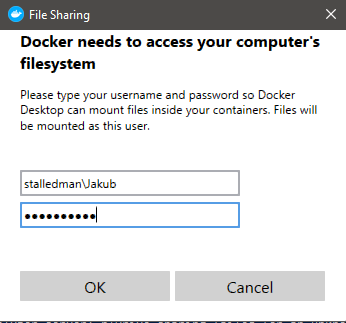
\includegraphics[width=0.5\linewidth]{instructions/docker3.PNG}
    \end{minipage}
    \item After command finishes executing, go to \url{http://localhost:8080/\#/examples/simulation-pipeline } in browser.
    \item To stop, press ctrl+c in \textit{PowerShell}
\end{enumerate}
\section{Linux}
\begin{enumerate}
    \item Install Docker using instructions from: \newline
    \url{https://docs.docker.com/install/}
    \item Install Docker Compose using official instructions from: \newline
    \url{https://docs.docker.com/compose/install/}
    \item Clone or download repository from: \newline
    \url{https://github.com/JakubSokolowski/simbad-monorepo}
    \item Open the terminal in the root folder of cloned repository
    \item Enter command docker-compose -f docker/prod-docker-compose.yml up. This will start the download process - this operation may take around 15 mins depending on the internet connection and will download around 4GB of data.
    \item Go to \url{http://localhost:8080/\#/examples/simulation-pipeline } in browser
    \item To stop, press ctrl+c in terminal
\end{enumerate}